\section{Introduction}

Dans ce chapitre nous allons présenter les techniques utilisées pour estimer les paramètres de la respiration du patient. Nous détaillerons tout d'abors les techniques permettant de connaître le signal respiratoire, qui est une grandeur très synthétique permettant d'estimer la position du patient sur le cycle respiratoire. Ensuite, nous présenterons les techniques permettant d'estimer le mouvement des organes au cours du cycle respiratoire.

\section{Estimation du signal respiratoire}

Le signal respiratoire est une grandeur caractérisant la position du patient sur le cycle respiratoire, entre la fin d'inspiration et la fin d'expiration. Il est habituellement fourni par des capteurs externes qui génèrent un signal corrélé avec la respiration. Cela permet de faire correspondre les données acquises par un imageur avec une phase particulière du mouvement respiratoire.

\subsection{Spiromètre}
\label{lab:spirometre}
Le spiromètre est un capteur externe placé sur la bouche du patient et qui permet de mesurer les déplacements d'air dans le système respiratoire~\cite{guivarc2004synchronization}. Les spiromètres mesurent un débit ou un volume d'air inspiré/expiré (voir illustration figure~\ref{fig:spirometre}). \`A partir de l'une des grandeurs (volume ou débit), il est possible d'estimer l'autre facilement. L'avantage du spiromètre est qu'il permet d'accéder à une mesure caractérisant directement la respiration du patient, et n'est pas sujet à des perturbations externes (mouvements involontaires par exemple). Par contre cela demande un appareillage qui peut être assez invasif pour le patient.

\begin{figure}[h!]
	\begin{center}
		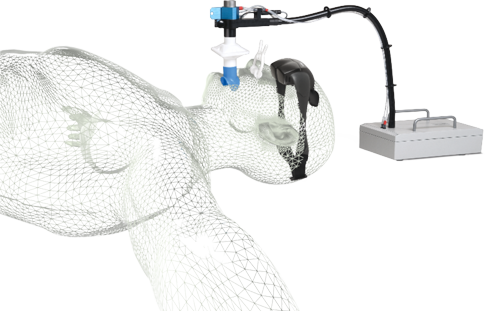
\includegraphics[width=12cm]{images/spiro}
	\end{center}
	\caption[Illustration du spiromètre Syn'r]{Illustration du spiromètre Syn'r : on peut voir le système de mesure de la respiration ainsi qu'un système de moniteurs implantés dans les lunettes pour aider le patient à contrôler sa respiration} 
	\label{fig:spirometre}
\end{figure}

\subsection{Ceinture}

Pour mesurer le signal respiratoire, il est possible d'utiliser un capteur qui va mesurer le périmètre du thorax. L'extension de cette ceinture va correspondre aux mouvements de la cage thoracique et de l'abdomen pendant la respiration du patient. C'est une mesure indirecte de l'amplitude du mouvement respiratoire utilisée couramment en routine clinique. 

Différentes technologies existent pour mesurer cette information (RespiTrace R250 de Studley. Data Systems, Respiratory Belt Transducer de ADInstruments, ...). Elles sont basées sur plusieurs effets (résisitif, inductif...) et ont l'avantage d'avoir un faible coût et de ne pas perturber le patient.

Bien qu'elles puissent être influencées par les mouvements involontaires du patient, il a été montré dans~\cite{Guivarch2004Sync} que les données acquises selon les méthodes par respiromètre et par ceinture sont équivalentes.

\subsection{Techniques basés sur des caméras vidéos}

Des caméras peuvent être utilisées pour estimer le mouvement respiratoire. Une des techniques consiste à utiliser des informations surfaciques en reconstruisant en 3D certaines parties du corps à l'aide de plusieurs caméras~\cite{beach2004feasibility}, ou en utilisant des caméras 3D temps de vol~\cite{fayad2009patient}. Cela permet d'avoir plus d'informations sur la respiration.

Une autre technique consiste à installer un marqueur sur le corps du patient et à relever les déplacements de ce marqueur selon plusieurs axes à l'aide d'une ou plusieurs caméra. Un tel système est décrit dans~\cite{nehmeh2002effect}. L'un de ces systèmes, le ``Respiratory Gating System'' de Varian Medical Systems est illustré sur  la figure~\ref{fig:RGSdeVarian}.

\begin{figure}[h!]
	\begin{center}
		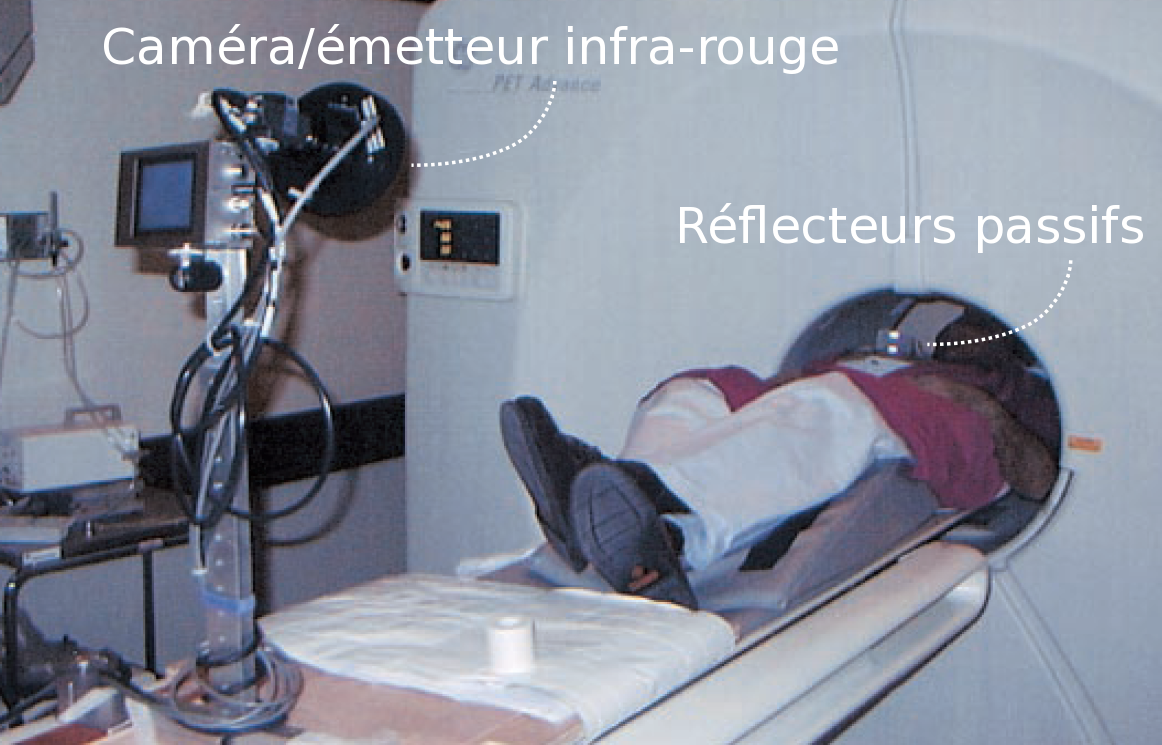
\includegraphics[width=12cm]{images/varian}
	\end{center}
	\caption[Photographie du système RGS de Varian medical Systems en action]{Photographie du système RGS de Varian medical Systems en action : une caméra va détecter le déplacement d'une zone du thorax en mesurant le déplacement de marqueurs placés sur un bloc plastique.} 
	\label{fig:RGSdeVarian}
\end{figure}

Ces techniques ont l'avantage d'être moins invasives et plus facilement acceptées par le patient. Cependant, elles sont beaucoup plus sensibles aux mouvements involontaires du patient. Ce risque est faible pour l'imagerie TDM car de faible durée (inférieure à la minute), mais il devient important pour les acquisitions TEP qui peuvent durer en tout plusieurs dizaines de minutes. Ces mouvements n'étant probablement pas corrélés avec le mouvement respiratoire, ils vont perturber le signal obtenu. 

\subsection{Techniques basées sur les images TEP}
\label{lab:estimMvtTEP}
En TEP, la publication de Bundschuh et al.~\cite{bundschuh2007postacquisition} utilise les données dynamiques pour estimer le signal respiratoire sans avoir besoin de capteur externe. Ce processus est réalisé en 5 étapes : 

\begin{enumerate}
 \item Les données TEP sont acquises en mode séquence (aussi appellé mode liste, défini en \ref{lab:modeliste}) : toutes les désintégrations détectées sont enregistrées dans un fichier de manière séquentielle.
 \item Une image TEP statique est reconstruite. Elle permet de localiser une lésion dans l'image qui servira d'amer pour l'estimation du mouvement respiratoire.
 \item Les données dynamiques sont regroupées en blocs de 0.5 secondes d'acquisitions. Chaque bloc est reconstruit séparément. 
 \item La zone d'intérêt choisie précédemment est sélectionnée dans chaque image reconstruite. La position axiale du barycentre à chaque instant temporel va donner une estimation du mouvement respiratoire pour le volume donné.
\end{enumerate}

Cette technique a été évaluée sur 10 patients et les signaux ont été comparés avec ceux obtenus avec des ceintures abdominales. Pour 3 patients, les courbes respiratoires obtenues par les deux techniques étaient très fortement corrélées. Pour deux autres patients, l'estimation de mouvement obtenue par la TEP était trop bruitée, mais montrait une bonne corrélation avec le signal obtenu par les ceintures abdominales après filtrage. Pour 3 autres patients, il n'a pas été possible de trouver une corrélation entre les deux signaux. Les deux derniers patients ont bougé pendant l'acquisition TEP, ce qui a perturbé le signal.

Cette technique est intéressante mais contrainte par la qualité de l'image TEP. En pratique, la moitié des acquisitions TEP n'a pas permis d'obtenir un signal respiratoire satisfaisant.


\section{Estimation du champ de mouvement}
\label{lab:estimChamp}

Le champ de mouvement est une information beaucoup plus riche que le signal respiratoire car il permet de suivre les déplacements des organes et des lésions à l'intérieur du corps du patient au cours d'un cycle respiratoire.

Le signal respiratoire acquis par les méthodes précédemment citées est utilisé pour décomposer les données acquises en TDM ou TEP en plusieurs phases, chacune correspondant à un instant du cycle. Ces informations sont utilisées pour rassembler les données acquises lors de chaque phase, reconstruites indépendamment. Ces reconstructions vont être utilisées pour estimer le champ de mouvement à l'aide de techniques de recalage.


\subsection{Image TEP 4D}
\label{lab:estimMvtTEP4D}
L'estimation du champ de mouvement respiratoire peut être faite à partir des données TEP, comme il a été montré par~\cite{dawood2008respiratory, dawood2006lung}. 

Les techniques utilisées sont analogues à celle présentée en~\ref{lab:estimMvtTEP}. Elles consistent à réaliser une acquisition séquentielle des données en même temps qu'une acquisition du signal respiratoire, puis à réorganiser les données acquises pour reconstruire les différents instants du cycle indépendamment et sans correction d'atténuation. Le mouvement est ensuite estimé à partir de ces images.

Pour obtenir le signal respiratoire, Dawood~\cite{dawood2008respiratory} utilise une caméra vidéo qui enregistre le mouvement d'un marqueur placé sur l'abdomen du patient. Ce marqueur est un point blanc placé sur un disque noir, et sa position axiale est détectée en calculant le barycentre des pixels dépassant une certain seuil. 

La synchronisation avec l'acquisition PET est réalisée à l'aide d'une LED située dans le champ de vue de la caméra qui s'allume lors du début de l'acquisition. Une fois l'acquisition terminée, le signal respiratoire obtenu par la caméra est utilisé pour répartir les évènements acquis par l'imageur TEP le long du cycle respiratoire. Ce cycle est décomposé en 8 parties qui seront reconstruites séparément, sans correction d'atténuation.

Les auteurs utilisent ensuite un algorithme de flux optique 3D présenté dans~\cite{dawood2006lung} et~\cite{horn1981determining} pour déterminer le champ de mouvement : Ils estiment un déplacement entre chaque image du cycle et l'image de référence correspondant à la quatrième phase (mi-expiration) dans le cas de cet article. Le résultat de l'algorithme est donc une séquence de champ de mouvement 3D,  formant un champ de déformation 4D.

L'algorithme a été testé sur le fantôme XCAT~\cite{segars2009mcatoverview} ainsi que sur les données de 16 patients. La performance de l'estimation de mouvement a été évaluée selon trois critères sur les images corrigées : la correction du déplacement axial du coeur, le coefficient de corrélation des images corrigées du mouvement, ainsi que le bruit obtenu. Ces résultats sont détaillés dans la présentation de cet article de la partie~\ref{lab:correctionDawood2008}.

Bai a présenté une technique d'estimation semblable~\cite{bai2009regularized}. L'étude a été réalisée sur des images simulées à l'aide du logiciel PET-SORTEO~\cite{reilhac2005pet} en utilisant le modèle NCAT~\cite{segars2009mcatoverview}, ainsi que sur une acquisition clinique. 24 lésions de fort contrastes (8:1) ont été introduites dans les modèles, pour une durée d'examen simulé de 10 minutes. L'erreur moyenne du diamètre longitudinal des lésions est très fortement améliorée par la correction, avec une erreur passant de 36\% à 16\% en moyenne sur l'ensemble des lésions. Le principe est le même que pour la publication précédente, à la différence que l'estimation de mouvement a été réalisée sur des images corrigées de l'atténuation à partir de la carte d'atténuation de la phase de référence. De plus, cette estimation du mouvement à été réalisée à l'aide d'une inteprolation par B-splines~\cite{thevenaz2000optimization}.

Un exemple de champ de déformation obtenu sur l'acquisition clinique est présenté en~\ref{fig:champMouvementBai}

\begin{figure}[h!]
	\begin{center}
		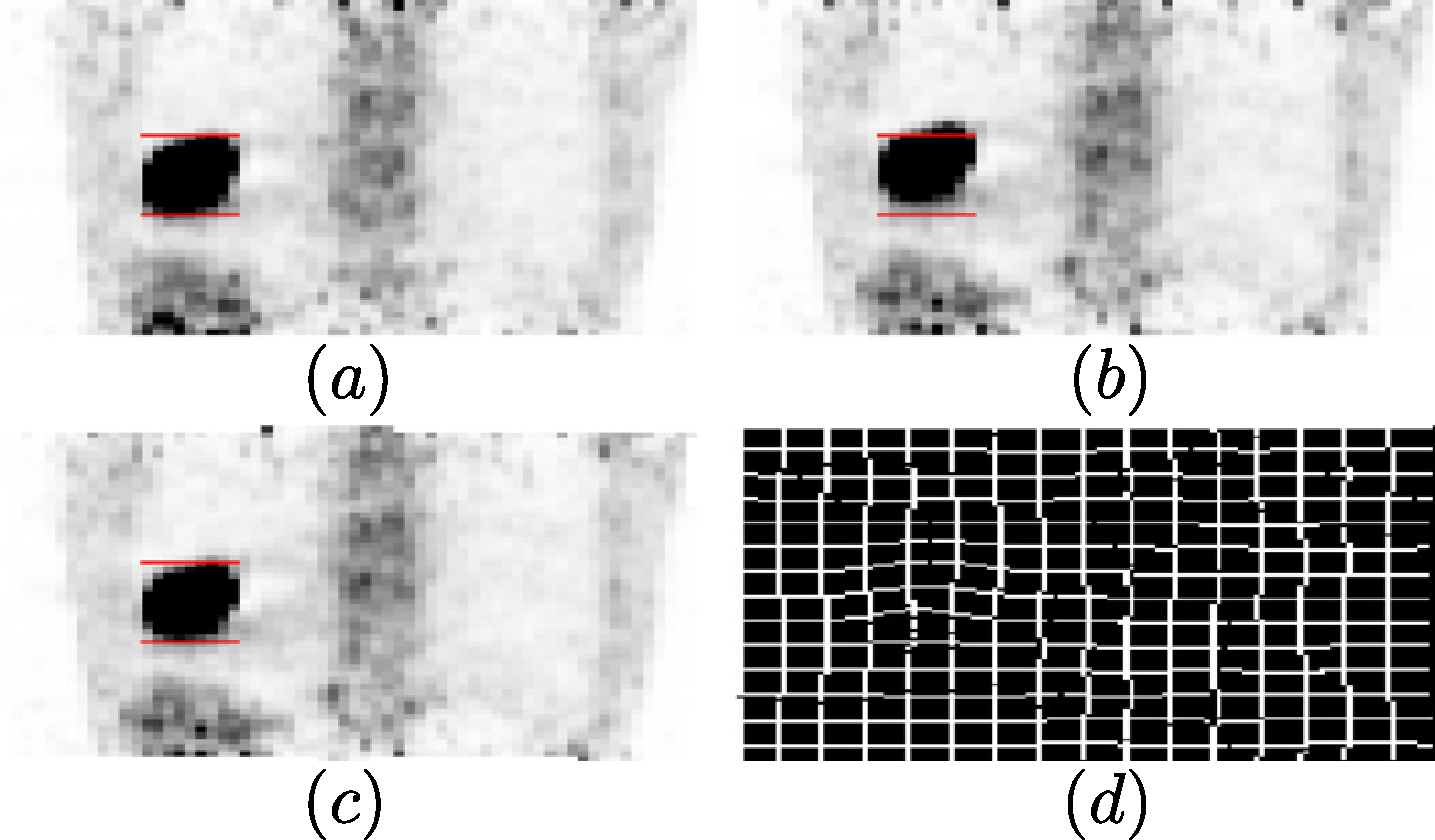
\includegraphics[width=12cm]{images/champDeformBai2}
	\end{center}
	\caption[Exemple de champ de mouvement]{Champ de déformation calculé sur des données cliniques à l'aide de la méthode présenté dans~\cite{bai2009regularized}. a) Image TEP obtenue à partir des données de la phase de référence  (mi-expiration), b) Image reconstruite pour les données d'expiration complète, et c) Résultat du recalage de l'image de fin d'expiration sur l'image de référence. d) représente le champ de mouvement résultat. Les traits rouges représentent l'extension axiale de la tumeur dans l'image de référence.} 
	\label{fig:champMouvementBai}
\end{figure}

\subsection{Image TDM 4D}

Les images TDM peuvent être acquises en mode dynamique de manière à obtenir une suite d'images couvrant tout le cycle respiratoire~\cite{lamare2007list, qiao2006motion}. Les données sont reconstruites indépendamment, avec un rapport signal sur bruit plus faible que sur l'image originale. 

Des algorithmes de recalage sont utilisés de manière à déduire le champ de mouvement. Le principal avantage de l'utilisation des images TDM 4D par rapport à la TEP est la précision des images. En effet, alors que les images TEP ont une résolution de l'ordre de 5mm, les images TDM atteignent des résolutions inférieures au mm, ce qui permet d'obtenir un champ de mouvement beaucoup plus précis. Cependant, utiliser des images TDM 4D a plusieurs inconvénients :

\begin{itemize}
 \item Une possible incohérence entre le cycle acquis en TDM 4D et la respiration du patient en TEP. Bien que les imageurs TEP/TDM couplent les deux sur la même machine, de manière à éviter les mouvements du patient entre les acquisitions, le cycle acquis en TDM ne représente qu'un cycle, tandis que l'acquisition TEP va donner un ``cycle moyen`` plus proche de la réalité.
 \item Une dose de radiation émise plus importante. Bien que les technologies récentes permettent de réduire les doses de manière importante pour l'acquisition dynamique, elles restent tout de même plus importante que pour un CT 3D.
\end{itemize}

Il faut noter que plusieurs publications basées sur des simulations se servent des cartes de labels utilisées par le simulateur pour réaliser les estimation de mouvement~\cite{lamare2007list}. Cela donne une estimation dans le ``meilleur des cas'', où l'image TDM est parfaitement en phase avec les images TEP. On utilise alors la méthode décrite précédemment pour estimer le champ de mouvement. L'intérêt de cette méthode est que les données anatomiques sont moins bruitées que les données TEP et contiennent plus d'information pour l'estimation des déformations. Cependant, l'acquisition d'un scanner TDM 4D en routine clinique peut être considérée comme très irradiante.

\subsection{Modèle}

Une autre voie en cours de développement est basée sur la création d'un modèle de respiration qui est adapté à chaque patient à partir d'une quantité réduite de données. Fayad~\cite{fayad2010application} propose un modèle basée sur l'analyse en composantes principales du champ de mouvement. 

Ce modèle est adapté à un patient à partir de deux images TDM prises à des instants différents du cycle, et d'un maillage dynamique de la surface du corps du patient obtenu pendant un cycle respiratoire complet. Dans son implémentation, le maillage est obtenu à l'aide d'une caméra vidéo temps de vol.

L'avantage de ce modèle est qu'il est totalement continu, et permet l'extraction d'un nombre arbitraire de phases sous la forme de matrices de déformation. Ce modèle a été testé sur des images simulées (2 fantômes XCAT) et 6 patients.

L'article \cite{vandemeulebroucke2009respiratory} présente une autre technique adaptée à l'imagerie TDM. Dans ce cas, un modèle est généré à partir d'une acquisitions TDM 4D en créant une image de mouvement moyenne, puis ce modèle est utilisé pour déduire le mouvement interne à partir d'accquisition de fluoroscopies en temps réel.